\documentclass{article}
\usepackage[T1]{fontenc}
\usepackage{lmodern}
\usepackage{graphicx}
\usepackage{amsmath,amssymb}
\usepackage[a4paper,margin=2cm]{geometry}
\usepackage[absolute,overlay]{textpos}
\setlength{\TPHorizModule}{1mm}
\setlength{\TPVertModule}{1mm}
\usepackage[indonesian]{babel}
\usepackage{hyperref}
\setlength{\emergencystretch}{2em}
% unit: Halaman 38

\begin{document}

% === Halaman 38 (llm) ===

Proses di bawah ini hanya menunjukkan pembangkitan $rk[1]$:

\begin{enumerate}
    \item $w[0] = (54, 77, 6F, 20)$; $w[1] = (4F, 6E, 65, 20)$; $w[2] = (4E, 69, 6E, 65)$; \\
    $w[3] = (20, 54, 77, 6F)$
    \item Mulai dari $i = 4$:
    \begin{enumerate}
        \item $temp = w[3]$
        \item $i = 4$ adalah kelipatan 4, maka jalankan fungsi g terhadap $w[3]$:
        \begin{itemize}
            \item Geser $w[3]$ satu $byte$ ke kiri secara sirkuler: $w[3] = (54, 77, 6E, 20)$
            \item Substitusi hasil pergeseran tersebut dengan $S\text{-}box$: $(20, F5, 9F, B7)$
            \item XOR-kan hasil di atas dengan $Rcon[1] = (01, 00, 00, 00)$, menghasilkan $(21, F5, 9F, B7)$
        \end{itemize}
        Jadi, $g(w[3]) = (21, F5, 9F, B7)$
        \item $w[4] = w[0] \oplus g(w[3]) = w[0] \oplus g(w[3]) = (75, 82, F0, 97)$
    \end{enumerate}

    Untuk $i = 5, 6, 7$:
    \[
    \begin{aligned}
    w[5] &= w[4] \oplus w[1] = (3A, EC, 96, B7), \\
    w[6] &= w[5] \oplus w[2] = (74, 85, F8, D2), \\
    w[7] &= w[6] \oplus w[3] = (54, D1, 8F, BD)
    \end{aligned}
    \]
\end{enumerate}

Dari proses di atas diperoleh $rk[1]$ sebagai berikut:

\vspace{10mm}

% deskripsi: Tabel hasil pembangkitan round key rk[1] yang terdiri dari nilai-nilai hexadecimal dalam grid 4x4.
% bbox normalisasi: [0.3240, 0.7980, 0.5940, 0.9410]
\begin{textblock*}{56.70mm}(68.04mm,237.01mm)
\noindent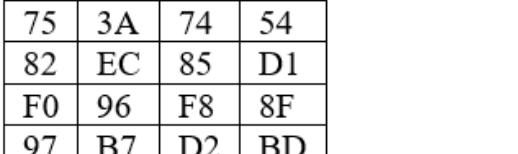
\includegraphics[width=56.70mm,height=42.47mm]{../../images/llm/page_038_img_01.png}%
\end{textblock*}

\end{document}
